% !TEX TS-program = pdflatex
% !TEX encoding = UTF-8 Unicode

% This is a simple template for a LaTeX document using the "article" class.
% See "book", "report", "letter" for other types of document.

\documentclass[11pt]{article} % use larger type; default would be 10pt

\usepackage[utf8]{inputenc} % set input encoding (not needed with XeLaTeX)
\usepackage{placeins}
\usepackage{listings}
%%% Examples of Article customizations
% These packages are optional, depending whether you want the features they provide.
% See the LaTeX Companion or other references for full information.

%%% PAGE DIMENSIONS
\usepackage{geometry} % to change the page dimensions
\geometry{a4paper} % or letterpaper (US) or a5paper or....
% \geometry{margin=2in} % for example, change the margins to 2 inches all round
% \geometry{landscape} % set up the page for landscape
%   read geometry.pdf for detailed page layout information

\usepackage{graphicx} % support the \includegraphics command and options

% \usepackage[parfill]{parskip} % Activate to begin paragraphs with an empty line rather than an indent
\usepackage{amsmath}
%%% PACKAGES
\usepackage{booktabs} % for much better looking tables
\usepackage{array} % for better arrays (eg matrices) in maths
\usepackage{paralist} % very flexible & customisable lists (eg. enumerate/itemize, etc.)
\usepackage{verbatim} % adds environment for commenting out blocks of text & for better verbatim
\usepackage{subfig} % make it possible to include more than one captioned figure/table in a single float
% These packages are all incorporated in the memoir class to one degree or another...

%%% HEADERS & FOOTERS
\usepackage{fancyhdr} % This should be set AFTER setting up the page geometry
\pagestyle{fancy} % options: empty , plain , fancy
\renewcommand{\headrulewidth}{0pt} % customise the layout...
\lhead{}\chead{}\rhead{}
\lfoot{}\cfoot{\thepage}\rfoot{}

%%% SECTION TITLE APPEARANCE
\usepackage{sectsty}
\usepackage{braket}
\allsectionsfont{\sffamily\mdseries\upshape} % (See the fntguide.pdf for font help)
% (This matches ConTeXt defaults)

%%% ToC (table of contents) APPEARANCE
\usepackage[nottoc,notlof,notlot]{tocbibind} % Put the bibliography in the ToC
\usepackage[titles,subfigure]{tocloft} % Alter the style of the Table of Contents
\renewcommand{\cftsecfont}{\rmfamily\mdseries\upshape}
\renewcommand{\cftsecpagefont}{\rmfamily\mdseries\upshape} % No bold!

%%% END Article customizations

%%% The "real" document content comes below...

\title{Projeect 2}
\author{Charles Loelius}
%\date{} % Activate to display a given date or no date (if empty),
         % otherwise the current date is printed 

\begin{document}
\maketitle

\section{Hamiltonian for Pair Conservation}

In this problem we consider a space of equally spaced single particle levels with a spin degeneracy(up and down spin). We can then consider a pair conserving Hamiltonian with a single particle part and a pairing term. We represent these as\\

\begin{equation}
H=H_0+V
\end{equation}

Where\\

\begin{equation}
H_0=\chi \sum_{p\sigma} \left(p-1\right)a_{p\sigma}^\dagger a_{p\sigma}
\end{equation}  

\begin{equation}
\braket{q_+q_-|V|s_+s_-} =-g \rightarrow V=-g\sum_{pq} a_{+p}^\dagger a_{p-}^\dagger a_{q+}a_{q-}
\end{equation}

Finally we define a pair creation and annhilation operator as\\
\begin{equation}\hat{P_p}=a_{p+} a_{p-}\end{equation}
\begin{equation}\hat{P_p}^\dagger=a_{p+}^\dagger a_{p-}^\dagger\end{equation}

From this it follows that\\

Now let us consider each of the commutation relations between the single particle and creation annhilation operators.\\

\begin{equation}
\left[P_p, P_q\right]=0
\end{equation}
\begin{equation}
\left[P_p,P_q^\dagger\right]=\delta_{p,q}
\end{equation}
\begin{equation}
\left[P_p,a_{q\sigma}\right]=0
\end{equation}
\begin{equation}
\left[P_p^\dagger,a_{q\sigma}\right]=-\delta_{p,q}a_{p-\sigma}^\dagger
\end{equation}
\begin{equation}
\left[P_p,a_{q\sigma}^\dagger \right]=\delta_{p,q}a_{p -\sigma}\end{equation}
\begin{equation}
\left[P_p^\dagger,a_{q \sigma}^\dagger \right]=0\end{equation}
\begin{equation}
\left[P_q^\dagger,P_p^\dagger\right]=0\end{equation}
We note that we can write V as \\
\begin{equation}
V=-g\sum_{pq}P_q^\dagger P_p \end{equation}



\subsection{$H_0,V$ commute with$S_z, S^2$}
\subsubsection{$H_0$ commutes with $S_z$}
\begin{equation}
\left[H_0,S_z\right]=\epsilon \sum_{p' \sigma' p\sigma} \left(p-1\right) \sigma' \left[a_{p\sigma}^\dagger a_{p\sigma},a_{p'\sigma'}^\dagger a_{p'\sigma'}\right]=A\left(\delta_{p,p'}\delta_{\sigma,\sigma'}-\delta_{p,p'}\delta_{\sigma,\sigma'}\right)=0\end{equation}
\subsubsection{$V$ commutes with $S_z$}
\begin{equation}
\left[V,S_z\right]=A\sum_{p,q,p',\sigma}\left[P_p^\dagger P_q,a_{p'\sigma}^\dagger a_{p\sigma} \right]=
\end{equation}\begin{equation}A\sum_{p,q,p',\sigma}\left(P_{p}^\dagger\left[P_{p},a_{p'\sigma}^\dagger \right]a_{p'\sigma}+P_p^\dagger a_{p'\sigma}^\dagger \left[P_p,a_{p'\sigma}\right]+\left[P_p^\dagger a_{p'\sigma}^\dagger \right]P_p,a_{p'\sigma}+a_{p'\sigma}^\dagger \left[P_p^\dagger,a_{p'\sigma}\right]P_p\right)
\end{equation}

\begin{equation}
= A\sum_{p,q,p'\sigma} \left(\delta_{p,p'}P_p^\dagger a_{p'-\sigma}a_{p'\sigma}-\delta_{p,p'}a_{p',\sigma}^\dagger a^\dagger_{p,-\sigma}P_p\right)=A\sum_{p\sigma} \left(P_p^\dagger P_p-P_p^\dagger P_p\right)=0\end{equation}


\subsubsection{$H_0$ commutes with $S^2$}

We note that \\
\begin{equation}
S^2=S_z^2+\frac{1}{2}\left(S_+S_- +S_-S_+ \right)
\end{equation}

Knowing from above that $H_0$ commutes with $S_z$ it thereby follows that  we must only prove\\

\begin{equation}
\left[H_0,\left(S_+S_- +S_-S_+ \right)\right]=0
\end{equation}

We note for any operator $O$ \\

\begin{equation}
\left[O,\left(S_+S_- +S_-S_+ \right)\right] =\left[O,S_+\right]S_-+\left[O,S_-\right]S_+ + S_+\left[O,S_-\right]+S_-\left[O,S_+\right]
\end{equation}


We then consider that $H_0$ is some constant  times $a_{p\sigma}^\dagger a_{p\sigma}$. Thus we consider that\\

\begin{equation}
\left[H_0,a_{p'\sigma'}^\dagger a_{p'-\sigma'}\right]=\sum_{p\sigma} (p-1) \left[a_{p\sigma}^\dagger a_{p\sigma},a_{p'\sigma'}^\dagger a_{p' -\sigma'} \right]=\end{equation}\begin{equation}\sum_{p\sigma} p(p-1) \delta_{p p'} \left(\delta_{\sigma \sigma'}a_{p' \sigma'}^\dagger a_{p\sigma}-\delta_{\sigma -\sigma'}\right)=0
\end{equation}

From this it immediately follows that \\

\begin{equation}
\left[H_0,S_\pm S_\mp\right]=0 \rightarrow \left[H_0,S^2\right]=0\end{equation}

\subsubsection{$\left[V,S_+S_-+S_-S_+=0\right]$	}

Again we take advantage of the general operator format, leading to\\
\begin{equation}
\resizebox{.9\hsize}{!}{$
\left[V,\left(S_+S_- +S_-S_+ \right)\right] =-g\sum_{pq} \left(\left[P_q^\dagger P_p ,S_+\right]S_-+\left[P_q^\dagger P_p ,S_-\right]S_+ + S_+\left[P_q^\dagger P_p,S_-\right]+S_-\left[P_q^\dagger P_p,S_+\right]\right)=$}
\end{equation}
\begin{equation}
\resizebox{.9\hsize}{!}{$
-g\sum_{pq} \left(\left(P_q^\dagger\left[ P_p ,S_+\right]+\left[ P_q^\dagger ,S_+\right]P_p\right)S_-+
\left(P_q^\dagger\left[ P_p ,S_-\right]+\left[P_q^\dagger,S_-\right]P_p\right)S_+ + S_+\left(P_q^\dagger \left[ P_p,S_-\right]+\left[P_q^\dagger,S_-\right]P_q^\dagger \right)+S_-\left(P_q^\dagger\left[ P_p,S_+\right]+\left[P_q^\dagger,S_+\right]P_p \right)\right)$}
\end{equation}

Next we consider\\

\begin{equation}
\left[P_p^\dagger , S_\sigma \right]=\left[P_p^\dagger, \sum_p a_{p\sigma}^\dagger a_{p-\sigma}\right]=
\sum_p' \left(\left[P_p^\dagger,  a_{p'\sigma}^\dagger \right]a_{p'-\sigma}+a_{p'\sigma}^\dagger \left[P_p^\dagger,a_{p'-\sigma}\right]\right)= -a_{p-\sigma}^\dagger a_{p\sigma}^\dagger
\end{equation}
\begin{equation}
\left[P_p , S_\sigma \right]=\left[P_p, \sum_p a_{p\sigma}^\dagger a_{p-\sigma}\right]=
\sum_p' \left(\left[P_p,  a_{p'\sigma}^\dagger \right]a_{p'-\sigma}+a_{p'\sigma}^\dagger \left[P_p,a_{p'-\sigma}\right]\right)= a_{p-\sigma} a_{p\sigma}
\end{equation}

Puting these together we are left with\\
\begin{equation}
\resizebox{.9\hsize}{!}{$
-g\sum_{pq} \left(\left(P_q^\dagger a_{p-}a_{p+} -a_{q-}^\dagger a_{q+}^\dagger  P_p\right)S_-+
\left(P_q^\dagger a_{p-}a_{p+}-a_{q-}^\dagger a_{q+}^\dagger P_p\right)S_+ + S_+\left(P_q^\dagger a_{p-}a_{p+}-a_{q-}^\dagger a_{q+}^\dagger P_p \right)+S_-\left(P_q^\dagger a_{p-}a_{p+}-a_{q-}^\dagger a_{q+}^\dagger P_p \right)\right)$}
\end{equation}

Substituting in $P_p$ we have \\

\begin{equation}
\resizebox{.9\hsize}{!}{$
-g\sum_{pq} \left(\left(P_q^\dagger P_p -P_q^\dagger  P_p\right)S_-+
\left(P_q^\dagger P_p -P_q^\dagger P_p\right)S_+ + S_+\left(P_q^\dagger P_p-P_q^\dagger P_p \right)+S_-\left(P_q^\dagger P_p-P_q ^\dagger P_p \right)\right)=0$}
\end{equation}







\subsection{Hamiltonian Commutes with $P_p^+ P_p^-$}

In order to show it keeps pairs together we must show that it conserves the product of the pair creation and annhilation operators. 


Now we can then take advantage of some basic commutator algebra to solve that\\

\begin{equation}
\left[P_p^\dagger P_p,P_q^\dagger P_r \right]=P_p^\dagger \left[P_p,P_q^\dagger\right]P_r+P_q^\dagger P_q^\dagger \left[P_p,P_r \right] +\left[P_p^\dagger,P_q^\dagger\right]P_r P_p+P_q^\dagger \left[P_p^\dagger, P_r \right]P_p\end{equation}\begin{equation}=\delta_{p,q}P_p^\dagger P_r -\delta_{p,r}P_q^\dagger P_p=P_q^\dagger P_r - P_q^\dagger P_r=0 \end{equation}

\begin{equation}
\left[P_p^\dagger P_p, a_{r \sigma}^\dagger a_{r\sigma}\right]=P_p^\dagger \left[P_p,a_{r\sigma}^\dagger\right]a_{r\sigma}+
P_p^\dagger a_{r\sigma}^\dagger \left[P_p,a_{r \sigma}\right] + \left[P_p^\dagger, a_{r\sigma}^\dagger \right] a_{r \sigma} P_p + a_{r \sigma}^\dagger \left[P_p^\dagger, a_{r \sigma} \right] P_p \end{equation}




\begin{equation}
\left[P_p^\dagger P_p, a_{r \sigma}^\dagger a_{r\sigma}\right]=P_p^\dagger\delta_{p,r} a_{p -\sigma} a_{r\sigma}-\delta_{p,r}a_{r\sigma}^\dagger a_{p-\sigma}^\dagger P_p=P_p^\dagger P_p-P_p^\dagger P_p =0\end{equation}

\section{Hilbert Space of Two Lowest Single Particle States, No Broken Pairs}

We can then establish first that $S=0$ and $S_z=0$. It thereby follows that \\

\begin{equation}
\hat{H}=a_{2+}^\dagger a_{2+}+a_{2-}^\dagger a_{2-}-g\left(P_1^\dagger P_1+P_1^\dagger P_2+P_2^\dagger P_1 + P_2^\dagger P_2 \right)\end{equation}

Now let us consider the case of the two eigenstates represented as \begin{equation}\psi=\begin{pmatrix} \psi_1 \\ \psi_2 \end{pmatrix}\end{equation}
Where the $\psi_i$ represents the states where a fermion pair is in state 1 or state 2. Then we have that\\

\begin{equation}
\hat{H}=\begin{pmatrix}  -g & -g \\ -g & -g+2 \end{pmatrix}\end{equation}

We see that this can be exactly solved for eigenvalues of\\

\begin{equation}
\left(-g-\lambda\right)\left(-g+2-\lambda\right)-g^2=\lambda^2+2g\lambda-2g-2\lambda=0 \end{equation}

So we have\\

\begin{equation}
\lambda=-g+1 \pm \sqrt{(g-1)^2+2g} \end{equation}

\section{Four Particles paired in p=1,2,3,4 states}

Here we see that a similar matrix can be constructed easily from the slater determinants.\\

Let us denote a state with pairs in states p=1, p=2 as $(1,2)$. Then we order these states as\\

\begin{equation}
\left[ (1,2), (1,3), (1,4), (2,3), (2,4), (3,4)\right]\end{equation}

We then construct the matrix in this order as(noting there are two combinations which will lead to the same bra and ket picking up a g term, and those where there are no overlaps will have none)

\begin{equation}\begin{pmatrix}
2-2g & -g & -g & -g & -g & 0\\
-g & 4-2g & -g & -g& 0 & -g\\
-g & -g & 6-2g & 0  & -g & -g \\
-g & -g & 0 & 6-2g & -g & -g\\
-g & 0 & -g & -g & 8-2g & -g\\
0& -g & -g & -g & -g & 10-2g
\end{pmatrix}
\end{equation}

We can now find the eigenvalues only numerically. 

\section{Code For Setting Up Matricies and Obtaining Eigenvalues}

In order to solve these problems, I have written a code which does a few things:
First, it takes an input basis of states which can be occupied. While used here for the base case of p,$\sigma$, it could be extended to any arbitrary quantum numbers. These can then be put into a hilbert space object, which orders and keeps track of the states, as well as generates the maximal Hilbert Space spanning this basis.\\

In order to restrict the basis a number of specific functions were also made, which determine if the sum of sigmas is 0 or if all states are paired. \\

At the heart of the machinery then are the creation and annhilation operators, which are constructed for each state. When applied to a Slater Determinant object, these return either 0 or a modified state vector (depending on what is appropriate.) With the help of an auxiliary function sort from the hilbert space, it is possible to then keep track of the phase as well. Finally, a Hamiltonian class incorporates these operators into one object which can then select a bra and ket to determine a matrix element from. This allows for the simple construction of a numpy matrix H for a given hilbert space(based on number of available quantum numbers, number of particles, pairing, etc.). This can easily be diagonalized using standard numpy algorithms, from which eigenvalues can be determined. In this case the single particle states were developed directly in the program. However, a generalization of the program to read in states from an input file would be trivial using numpy.genfromtxt.\\

In order to compare the results, I show below the resulting eigenvalues generated from the 4 p states 4 particle states and 6 ps states 6 particle states.\\

For g=0 we see immediately we have in the 4p state case\\
\begin{equation}
E=\left[2,8,10,6,6,4\right] \end{equation}

We see these match exactly with the values from the above matrix(which is diagonal with g=0). 

We can also consider the degenerate case where we allow the energy of all states to be 1. This leads to in the case of the 4 particles and 4 p states to a diagonal matrix $4I$, which just counts the particles in each state. Allowing now g=1 and $H_0$ to be 0 we have eigenvalues of \\
\begin{equation}
E=\left[-6,-2,-2,0,0\right]\end{equation}

We know from the base case of degeneracy that as the degeneracy is 4 in p and 2 in spin and so totals to 8 states, and such we should expect a ground state of \\
\begin{equation}
E_0=-\frac{g}{4}n\left(\Omega-n+2\right)=-\left(8-4+2\right)=-6\end{equation}

We see the program's results agree with the prediction. \\
\section{Varying g}

For the larger scale cases the program takes more time to run. To that end I designed a function to run through a number of values for g in a given hilbert space, forming Hamiltonians, and from there calculating the matricies, finding their eigenvalues and graphing each of these on a scatterplot vs g. The results of this are shown below.
\FloatBarrier
\begin{figure}[hbt!]
\centering
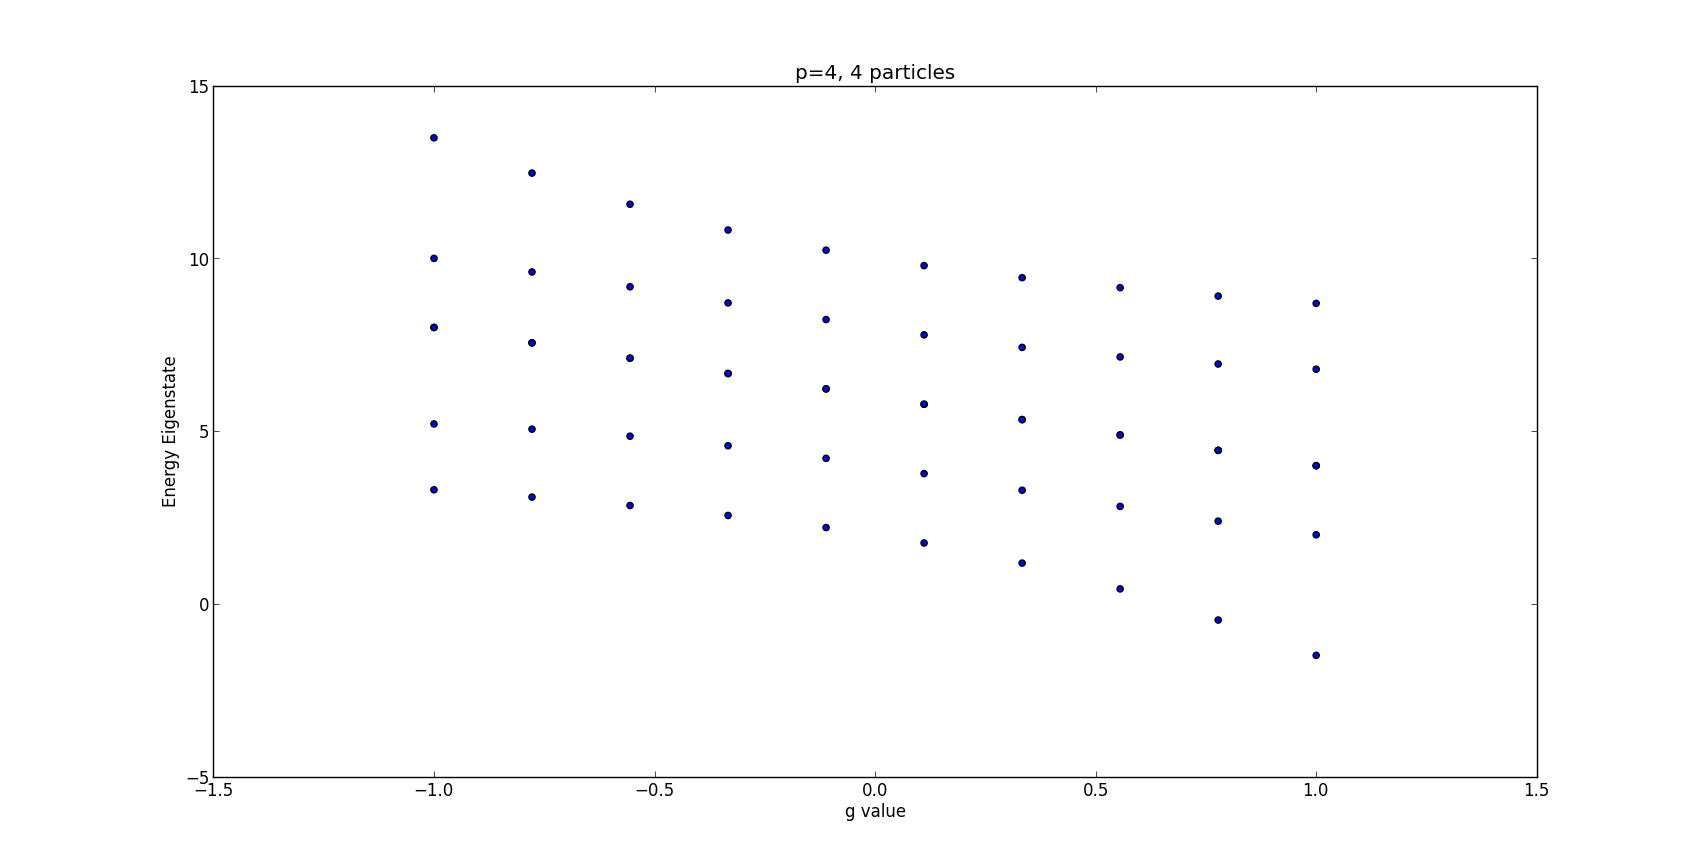
\includegraphics[width=.7\linewidth]{p4p4}
\caption{Effect of changing g on energy eigenstates for 4 particles and states}
\end{figure}
\FloatBarrier

\FloatBarrier
\begin{figure}[hbt!]
\centering
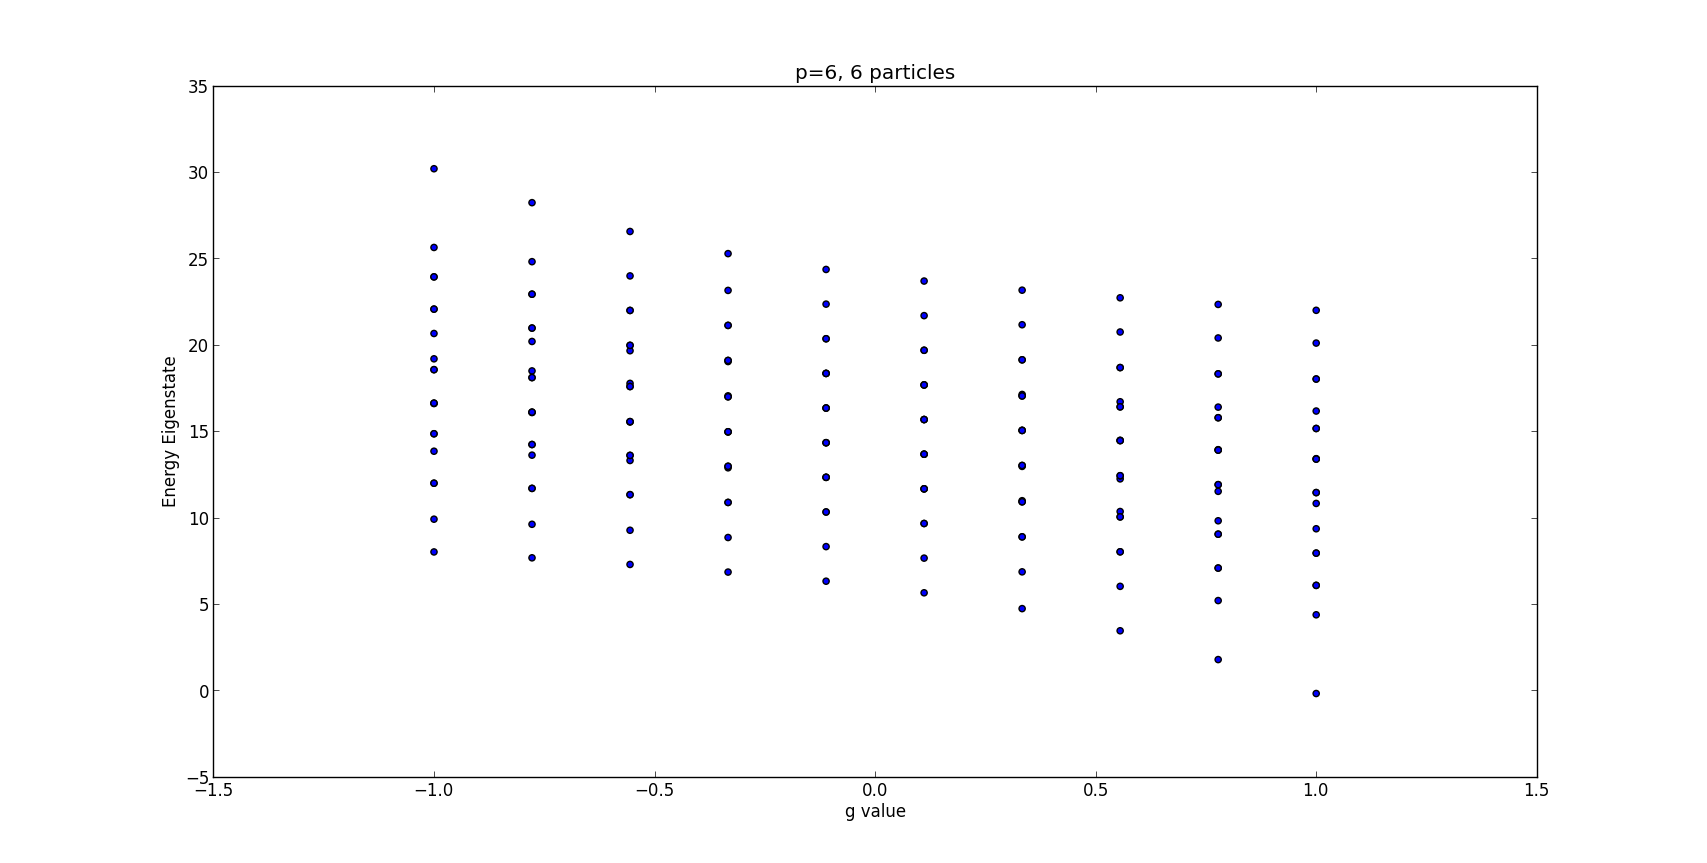
\includegraphics[width=.7\linewidth]{p6p6}
\caption{Effect of changing g on energy eigenstates for 6 particles and states}
\end{figure}
\FloatBarrier


\FloatBarrier
\begin{figure}[hbt!]
\centering
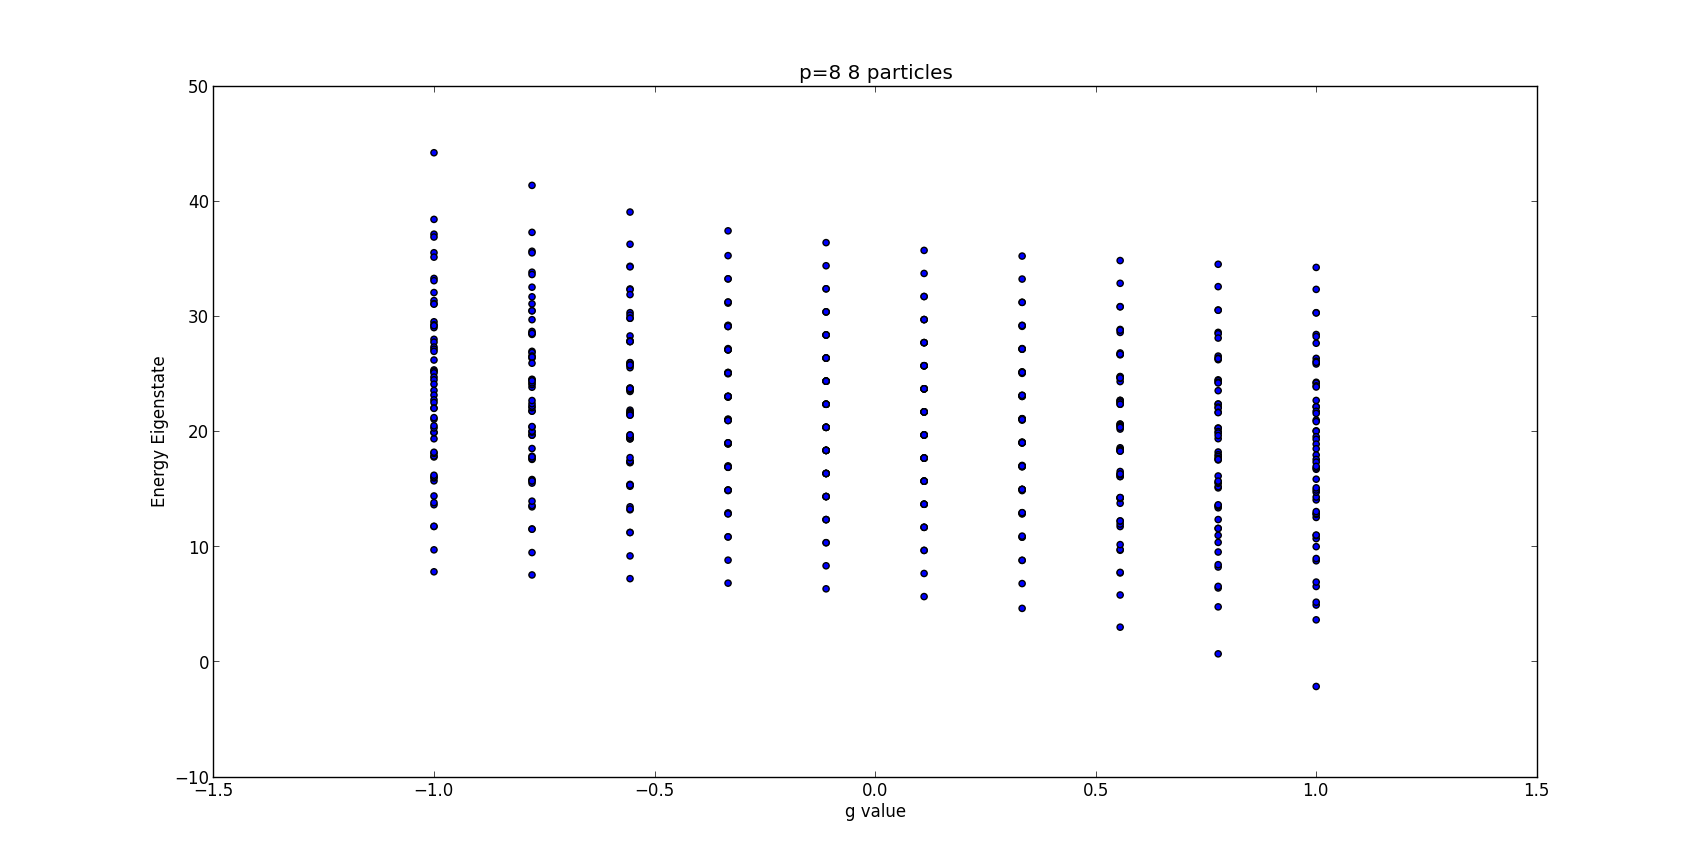
\includegraphics[width=.7\linewidth]{p8p8}
\caption{Effect of changing g on energy eigenstates for 8 particles and states}
\end{figure}
\FloatBarrier

We note that while the proliferation of energy states with a larger number of levels and states is a striking feature, it is of course expected. What we may note of more interest, perhaps, is that there is a lifting of degeneracies as g becomes larger, for example there are 10 clearly visible states near g=0 for six particles and states, but 13 energy states near g=1. A similar pattern is clear for the 8 particles and states. We also note that the energy shifting is not equal among all energies, but that for large g the ground state is shifted much lower than the highest state, compared to g=0, and similarly at $g\approx -1$ the reverse holds true, with the highest state showing a vast shift upwards. 

\section{Code}
\subsection{Module}
\lstinputlisting[language=Python]{C:/pyzo2013b/Lib/ShellModel.py}
\subsection{Implementation}

\lstinputlisting[language=Python]{Project2Implementation.py}



%
%\begin{equation}
%\left[P_p^\dagger P_p ,V\right]=-g \sum_{ab} P_a^\dagger P_b P_p^\dagger P_p +gP_p^\dagger P_p\sum_{ab}P_a^\dagger P_b
%\end{equation}
%
%Now we note for all cases where $a,b \neq b$ it follows that the pair operators commute with the terms and so those terms cancel. Furthermore in the case where $a=b=p$ there is a trivial commutation. We are thus left with only the term where $a=p, b\neq p$ or $b=p, a \neq p$.\\
%
%In the first of the cases we thus have, using standard commutator algebra and remembering that $p\neq b$.\\
%
%\begin{equation}
%\left[P_p^\dagger P_p, P_p^\dagger P_b \right]= P_p^\dagger \left[P_p,P_p^\dagger\right]P_b +P_p^\dagger P_p^\dagger \left[P_p,P_b\right]+\left[P_p^\dagger,P_p^\dagger\right]P_p P_b+P_p^\dagger \left[P_p^\dagger,P_b\right] P_p=P_p^\dagger \left[P_p,P_p^\dagger\right]P_b\end{equation}
%
%And doing the same for the second we have\\
%\begin{equation}
%\left[P_p^\dagger P_p, P_a^\dagger P_p \right]= P_p^\dagger \left[P_p,P_a^\dagger\right]P_p +P_p^\dagger P_a^\dagger \left[P_p,P_p\right]+\left[P_a^\dagger,P_p^\dagger\right]P_p P_p+P_a^\dagger \left[P_p^\dagger,P_p\right] P_p=P_a^\dagger \left[P_p^\dagger,P_p\right]P_p=-P_a^\dagger \left[P_p,P_p^\dagger\right]P_p\end{equation}
%
%Finally we note that the commutator $\left[P_p^\dagger,P_p \right]$ is just 1 looking at the commutator of the individual creation and annhilation operators. As we are summing over all a and b that each of these variables is a dummy variable and so all of these commutators summed will go to zero. As such the Hamiltonian commutes with the pair operator. 

\end{document}
